% This is based on the LLNCS.DEM the demonstration file of
% the LaTeX macro package from Springer-Verlag
% for Lecture Notes in Computer Science,
% version 2.4 for LaTeX2e as of 16. April 2010
%
% See http://www.springer.com/computer/lncs/lncs+authors?SGWID=0-40209-0-0-0
% for the full guidelines.
%
\documentclass{llncs}

\usepackage{graphicx}
\usepackage{verbatim}
\usepackage{fancyhdr}
\usepackage{listings}
\usepackage{color}
\usepackage{booktabs}

\definecolor{dkgreen}{rgb}{0,0.6,0}
\definecolor{gray}{rgb}{0.5,0.5,0.5}
\definecolor{mauve}{rgb}{0.58,0,0.82}

\lstset{frame=tb,
  language=Prolog,
  aboveskip=3mm,
  belowskip=3mm,
  showstringspaces=false,
  columns=flexible,
  basicstyle={\small\ttfamily},
  numbers=none,
  numberstyle=\tiny\color{gray},
  keywordstyle=\color{blue},
  commentstyle=\color{dkgreen},
  stringstyle=\color{mauve},
  breaklines=true,
  breakatwhitespace=true,
  tabsize=3
  }

\begin{document}

\title{Skyscraper}
%
\titlerunning{Skyscraper}  % abbreviated title (for running head)
%                                     also used for the TOC unless
%                                     \toctitle is used
%
\author{André Cruz\inst{1} \and Edgar Carneiro\inst{2}}
%
\authorrunning{André Cruz \and Edgar Carneiro} % abbreviated author list (for running head)
%
%%%% list of authors for the TOC (use if author list has to be modified)
\tocauthor{André Cruz and Edgar Carneiro}
%
\institute{Faculdade de Engenharia da Universidade do Porto\\ Rua Roberto Frias, sn, 4200-465 Porto, Portugal,\\
\email{ feup@fe.up.pt},\\ WWW home page:
\texttt{http://www.fe.up.pt}}

\maketitle              % typeset the title of the contribution

\begin{abstract}
This article was written for the course unit ``Logic Programming'', from the course Master in Informatics and Computing Engineering.
This article purpose is to present how the program we developed is able to solve the decision problem that is the puzzle Skyscraper, independently of board size.
The program developed is also able to generate Skyscraper puzzles as well. The program developed uses Logic Programming with Constraints as the approach to solve and generate the puzzles.
\keywords{skyscraper, CLP, sicstus, PLOG, FEUP}
\end{abstract}
%
\section{Introduction}
%
The main purpose of this project was to develop a program that would be able to solve either Decision Problems or Optimization Problems, by using Logic Programming with Constraints.

Our group was assigned with a decision problem: the Skyscraper puzzle. Succinctly, the puzzle consists of a grid that the player needs to fill, according to some given restrictions, and without repeating the same digits per column and per row.

The article approaches several topics such as: what were the variables used and its domains, what were the constraints used and their implementation in the program, what is the labeling strategy implemented, what are the results of the developed program and what are the final conclusions obtained from developing the project.

%
\section{Problem Description}
%
Skyscraper consists of a puzzle where the player needs to fill a grid with digits from 1 to \textit{N} --- with \textit{N} being the size of the grid --- where each row and column contains each digit exactly once. In the grid, each number represents the height of a building. The numbers outside the grid indicate how many buildings can be seen when looking from that direction. Taller buildings block the view of smaller buildings meaning that every number beyond a number bigger than it will not be taken into account, when looking from that direction.

The difficulty of the puzzle arises from the conjugation of two factors: the digits in rows and columns must all be distinct and the restrictions outside the grid.

\begin{figure}[h!]
\begin{center}
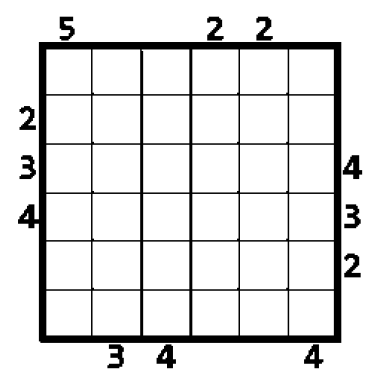
\includegraphics[height=4.5cm,width=4.5cm]{images/skyscraper_unsolved.png}
\caption{Unsolved 6x6 Skyscraper puzzle}
\label{Figure 1}
\end{center}
\end{figure}

\begin{figure}[h!]
\begin{center}
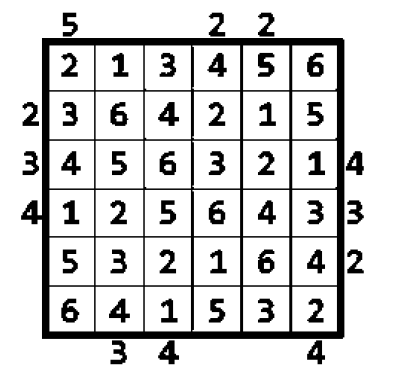
\includegraphics[height=4.5cm,width=4.5cm]{images/skyscraper_solved.png}
\caption{Solved 6x6 Skyscraper puzzle}
\label{Figure 2}
\end{center}
\end{figure}

%
\section{Approach}

In the implementation of Skyscraper in Prolog, the group used a list of lists to represent the grid. The value of each element will correspond to the height of the building it represents.
Elements whose value is not known will be represented by  a `\_', therefore representing in Prolog non- instantiated values.

For the restrictions outside the grid, the group also decided to use a list of lists. The list containing the other lists will always have length four since each one of its elements is a list containing the restrictions of the correspondent border. The order by which the border's restrictions are kept in the list is: Top border restrictions, Left border restrictions, Bottom border restrictions and Right border restrictions. If the restriction for a certain row or column does not exist, a `0' is used in its representation.

\begin{figure}[h!]
\begin{center}
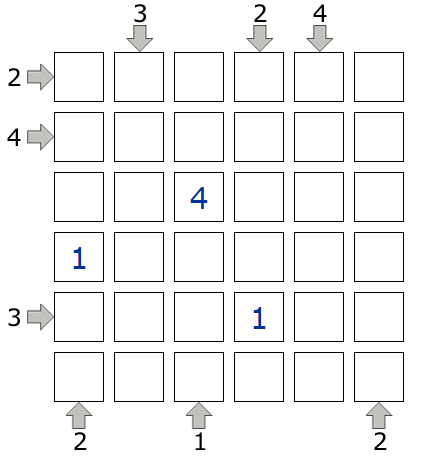
\includegraphics[height=5cm,width=5cm]{images/example_skyscraper.png}
\caption{Example of a skyscraper puzzle followed by its Prolog representation}
\label{Figure 3}
\end{center}
\end{figure}
\noindent\begin{minipage}{.48\textwidth}
\begin{lstlisting}[frame=tlrb, caption=Prolog grid representation]
testBoard([
  [_, _, _, _, _, _],
  [_, _, _, _, _, _],
  [_, _, 4, _, _, _],
  [1, _, _, _, _, _],
  [_, _, _, 1, _, _],
  [_, _, _, _, _, _]
]).
\end{lstlisting}
\end{minipage}\hfill
\begin{minipage}{.42\textwidth}
\begin{lstlisting}[frame=tblr, caption=Prolog representation of border restrictions]
testRestrictions([
  [0, 3, 0, 2, 4, 0],
  [2, 4, 0, 0, 3, 0],
  [2, 0, 1, 0, 0, 2],
  [0, 0, 0, 0, 0, 0]
]).
\end{lstlisting}
\end{minipage}\hfill

%
\subsection{Decision Variables}

The decision variables associated with a skyscraper puzzle are: the lists representing the rows of the grid. Since all the elements in a row and column must have a different value --- as it is a skyscraper rule --- the domain of the elements in each row will have to be defined between 1 and the length of the board, \textit{N}, and they will also have to be all distinct. The following code presents the application of the referred restrains to the decision variables.\\

\noindent\begin{minipage}{.44\textwidth}
\begin{lstlisting}[frame= tblr, caption=Row domain restrictions]
restrictBoardDomain([], _).
restrictBoardDomain([Row | Board], N) :-
  length(Row, N),
  domain(Row, 1, N),
  all_distinct(Row),
  restrictBoardDomain(Board, N).
\end{lstlisting}
\end{minipage}\hfill
\begin{minipage}{.5\textwidth}
\begin{lstlisting}[frame=tblr, caption=Column all elements distinct]
all_distinct_columns(_, 0) :- !.
all_distinct_columns(Board, N) :-
  N > 0, !,
  getBoardCol(Board, N, Col),
  all_distinct(Col),
  NewN is N - 1,
  all_distinct_columns(Board, NewN).
\end{lstlisting}
\end{minipage}\hfill

\textbf{TODO} Os side domains tb sao? penso que nao porque nao queremos instanciar nada ai... although it seems in code

%
\subsection{Constraints}

The restrictions defined for the puzzle are the ones from the rules. The rules that force the inexistence of repeated elements in either a row or a column were already implemented by the way the domains are defined (see section \textbf{Decision Variables}). Therefore, the challenge involving the project was the addition of PROLOG restrictions to implement the missing rule: assuring that the number outside the grid would indeed control the number of `visible buildings'.\\

Theoretically, what we needed to implement in order to achieve the last rule was an IF CLAUSE, being that: if the element is bigger than the maximum value so far, than the element is the new maximum value, and the elements correspondent building is visible, otherwise, the building is not visible and the maximum value stays the same. However, since in Constraints  Logic Programming the elements value would not be instantiated this implementation proved hard. \textbf{Um bcd bullshit este texto, mudar? xD ou mm apagar}

The solution we came up to implement that last rule was a \textit{logic XOR (\textbf{\#\textbackslash})}, because the element being analyzed was either a maximum value and the number of visible buildings would increment, or it was not and the count of visible buildings would stay the same. In the end, we wanted to, when the line was finished being analyzed, the number of visible buildings would be equal to the corresponding border restraining value. The predicate would be called for each line/ column for each of the four possible directions: left to right, right to left, top to bottom and bottom to top. 

\begin{lstlisting}[frame=tblr, caption=Constraint that assures correct number of visible buildings ]	
/**
 * Apply restrictions to Row.
 * +Predicate Order in which elements are analyzed - fetches an element.
 * +Num is the number of visible skyscrapers according to the above order.
 */
applyToRow(Num, Row, Max, GetElement) :-
  call(GetElement, Row, El, RemainderRow),
  NewNum #>= 0,
  (El #> Max #/\ NewMax #= El #/\ NewNum #= Num - 1) #\/
  (El #=< Max #/\ NewMax #= Max #/\ NewNum #= Num),
  applyToRow(NewNum, RemainderRow, NewMax, GetElement).
applyToRow(0, [], _, _).
\end{lstlisting}

%
\subsection{Evaluation Function}

In Skyscraper there is no evaluation of solutions, since the puzzle is solved whenever a solution is found.

%
\subsection{Search Strategy}

The labeling strategy implemented in the program was the \textbf{\textit{ffc}}, also known as \textit{most\_constrained}. This labeling strategy makes use of the most constrained heuristic: ` a variable with the smallest domain is selected, breaking ties by (a) selecting the variable that has the most constraints suspended on it and (b) selecting the leftmost one'[3].  We opted for this heuristic as it would be the one providing faster and more efficient solutions for the skyscraper puzzle. This was natural having in mind the kind ofconstraints that were applied during the development, namely the constraint that assure the building heights were correct,\textbf{ver a frase a partir daqui :/} that is: since the entire board is not instantiated the solution will be faster if the first most constrained values --- therefore the ones most unlikely to wrong --- are first discovered and snowball from there on.

%
\section{Solution Presentation}

For the solution presentation in text mode the predicate \textit{printBoard} is used. If run as \textbf{\textit{printBoard(+Board)}}, it only prints the given board in a user friendly way. However, if run as \textbf{\textit{printBoard(+Board, +Restrictions)}} it will print the board in a user friendly way while also displaying the boarder restrictions being applied to each row or column. The predicate makes use of helper predicates such as \textbf{\textit{printRow(+Row)}}, that prints the given row and \textbf{\textit{printHBorder(+Length)}}, that prints the horizontal border at the top and the bottom. All this predicates are defined in the file \textbf{\textit{display.pl}}.

\begin{figure}[h!]
\begin{center}
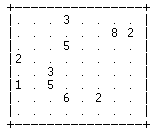
\includegraphics[height=3cm,width=3cm]{images/printBoard1.png}
\caption{Example of a call to printBoard/1}
\label{Figure 3}
\end{center}
\end{figure}

\begin{figure}[h!]
\begin{center}
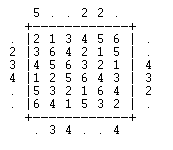
\includegraphics[height=4cm,width=4cm]{images/printBoard21.png}
\caption{Example of a call to printBoard/2 with a solved board}
\label{Figure 4}
\end{center}
\end{figure}

%
\section{Results}

The group tried to make extensive and exhaustive tests to be able to conclude fiercely about the given results.

The results of several tests that the group made the program went through were:

\begin{table}[]
\centering
\caption{Each of the values is the result of the average of several tests made}
\label{Results Tablel}
\begin{tabular}{@{}ccc@{}}
\toprule
\multicolumn{1}{c|}{\textbf{Board Size}} & \multicolumn{1}{c|}{\textbf{Time /s}} & \textbf{Backtracks} \\ \midrule
4x4                                      & 0.0                                 & 9                   \\ \midrule
5x5                                      & 0.047                                 & 659                 \\ \midrule
6x6                                      & 0.291                                 & 5438                \\ \midrule
7x7                                      & 10.489                                & 159196              \\ \midrule
8x8                                      & 18.239                                & 315893              \\ \bottomrule
\end{tabular}
\end{table}

In the end, the conclusions the group came up with were:
\begin{itemize}
	\item There is an exponential relation between the board size and time taken to solve the puzzle. For smaller boards the difference in board size affects slightly the difference of times (board size 4 to baoard size 5, differences of around 0.05s). However in bigger boards the difference of board sizes affect time fiercely (board size 6 to board size 7, differences of around 10s).

\begin{figure}[h!]
\begin{center}
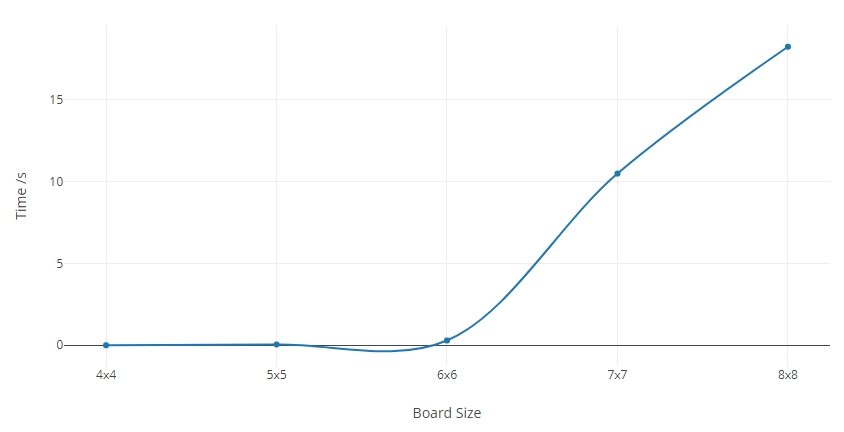
\includegraphics[height=6cm,width=12cm]{images/graph1.png}
\caption{Relation between board size and time to solve the puzzle}
\label{Figure 5}
\end{center}
\end{figure}

	\item There is a strong correlation between the number of backtracks (and the other statistics, such as \textit{Resumptions, Entailments, Prunings and Constraints created}) and time. The higher the alue of the statistics the higher the tame ita took the program to solve the puzzle.

\begin{figure}[h!]
\begin{center}
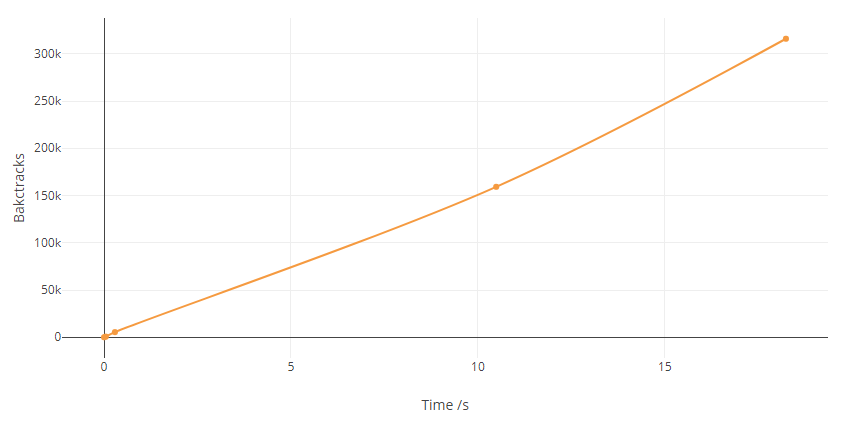
\includegraphics[height=6cm,width=12cm]{images/graph2.png}
\caption{Relation between number of backtracks and time to solve the puzzle}
\label{Figure 6}
\end{center}
\end{figure}
	
	\item Also worth notice, despiting not being visible in the table because its values are an average, is the fact that puzzle with a higher number of border restricitons are faster to solve. This is naturally explained since the information received by the solver is bigger and therefore the number of backtracks done is smaller.
\end{itemize}

%
\section{Conclusion and Future Work}

We believe that our knowledge about Logic Programming was deeply increased, with everything we had proposed to do being accomplished in the required time.

The program developed has no limitations regarding board size or problem generation, despite becoming slower with bigger board sizes. Therefore, the only way possible to improve the developed application would be by improving the solver efficiency and time. However, the group tried fiercely to make that improve by trying out several approaches but in the end, the best solution was the one being presented.

The group also agreed in the fact that Logic Programming with Constrains revealed itself to be an extremely powerful tool, able to solve easily certain problems (such as the one this work is based in) that would take much more time and effort to solve with other paradigms.\\

To sum up, despite Logic Programming with Constraints being a totally different paradigm from what the group had ever worked with, we quickly got used to it and learnt to appreciate the cons and pros that it presents, thus having it culminate in a project we are proud of.

%


%
% ---- Bibliography ----
%
\begin{thebibliography}{5}
%
\bibitem {ster:shap:warr}
L. Sterling, E. Y. Shapiro, and D. H. D. Warren, The Art of Prolog: Advanced Programming Techniques. MIT Press, 2010.

\bibitem {carl:fru}
M. Carlsson and T. Fruhwirth, SICStus Prolog User's Manual. SICS Swedish ICT AB, 4.3.5 ed., 2016.

\bibitem {sky}
Skyscraper rules,
http://logicmastersindia.com/lmitests/dl.asp?attachmentid=659\&view=1

\end{thebibliography}

\clearpage

\appendix

\section{Appendix}

\huge\textbf{skyscraper.pl}
\begin{lstlisting}[language=Prolog]
:- include('solver.pl').
:- include('display.pl').
:- include('test_data.pl').
:- include('generator.pl').

%Predicate to run the default puzzle
skyscraper :-
  nl, write('Skyscraper!'), nl, nl,
  testRestrictions(R),
  R = [Up | _Rest],
  length(Up, Size),
  solveBoard(Size, B, R),
  printBoard(B, R).
\end{lstlisting}
\newpage

\huge\textbf{solver.pl}
\begin{lstlisting}[language=Prolog]
:- use_module(library(clpfd)).
:- use_module(library(lists)).

/**
 * Domain restriction
 */
sidesDomain(Size, [List | Rest]) :-
  length(List, Size),
  domain(List, 0, Size),
  sidesDomain(Size, Rest).
sidesDomain(_, []).

restrictBoardDomain([], _).
restrictBoardDomain([Row | Board], N) :-
  length(Row, N),
  domain(Row, 1, N),
  all_distinct(Row),
  restrictBoardDomain(Board, N).

all_distinct_columns(_, 0) :- !.
all_distinct_columns(Board, N) :-
  N > 0, !,
  getBoardCol(Board, N, Col),
  all_distinct(Col),
  NewN is N - 1,
  all_distinct_columns(Board, NewN).


% Get the nth1 column of the given Board (1 indexed)
getBoardCol([], _, []).
getBoardCol([Row | Board], N, [El | Col]) :-
  element(N, Row, El),
  getBoardCol(Board, N, Col).


%% Gets the FIRST element of a given row
getFirstElement([Element | RemainderRow], Element, RemainderRow).

%% Gets the LAST element of a given row
getLastElement(Row, Element, RemainderRow) :-
  append(RemainderRow, [Element], Row).


%% LEFT to RIGHT
applyLeftToRight(Num, Row) :-
  applyToRow(Num, Row, 0, getFirstElement).

%% RIGHT to LEFT
applyRightToLeft(Num, Row) :-
  applyToRow(Num, Row, 0, getLastElement).

/**
 * Apply restrictions to Row.
 * +Predicate Order in which elements are analyzed - fetches an element.
 * +Num is the number of visible skyscrapers according to the above order.
 */
applyToRow(Num, Row, Max, GetElement) :-
  call(GetElement, Row, El, RemainderRow),
  NewNum #>= 0,
  (El #> Max #/\ NewMax #= El #/\ NewNum #= Num - 1) #\
  (El #=< Max #/\ NewMax #= Max #/\ NewNum #= Num),
  applyToRow(NewNum, RemainderRow, NewMax, GetElement).
applyToRow(0, [], _, _).

/**
 * Applies restrictions Horizontally along the board
 * +Predicate is the predicate used to apply restrictions on the fetched Row.
 */
applyAllHorizontalRestrictions([0 | Rest], [_ | Rows], Predicate) :-
  applyAllHorizontalRestrictions(Rest, Rows, Predicate).
applyAllHorizontalRestrictions([N | Rest], [Row1 | Rows], Predicate) :-
  call(Predicate, N, Row1),
  applyAllHorizontalRestrictions(Rest, Rows, Predicate).
applyAllHorizontalRestrictions([], [], _).

/**
 * Applies restrictions Vertically along the board
 * +Predicate is the predicate used to apply restrictions on the fetched Column.
 */
applyAllVerticalRestrictions(Restrictions, Board, Predicate) :-
  applyAllVerticalRestrictions(Restrictions, Board, Predicate, 1).
applyAllVerticalRestrictions([0 | Rest], Board, Predicate, Count) :-
  NewCount is Count + 1,
  applyAllVerticalRestrictions(Rest, Board, Predicate, NewCount).
applyAllVerticalRestrictions([N | Rest], Board, Predicate, Count) :-
  NewCount is Count + 1,
  getBoardCol(Board, Count, Col),
  call(Predicate, N, Col),
  applyAllVerticalRestrictions(Rest, Board, Predicate, NewCount).
applyAllVerticalRestrictions([], _, _, _).


/**
 *  +Sides -> a list of lists, each of which represents the restrictions on the side of the board (number of visible buildings).
 *      -> in order: [TopRestrictions, LeftRestrictions, BottomRestrictions, RightRestrictions]
 *      -> elements of list are in range [0,N], 0 meaning an undefined restriction
 *      -> elements correspond to restrictions in top->bottom (left/right lists) or left->right (top/bottom lists) order
 *  -Board -> a list of lists (a matrix)
 */
solveBoard(Size, Board, Sides) :-
  Sides = [Top, Left, Bottom, Right],
  sidesDomain(Size, Sides),

  % Domain
  length(Board, Size),
  restrictBoardDomain(Board, Size),
  all_distinct_columns(Board, Size),

  % Apply restrictions to board rows/columns
  applyAllHorizontalRestrictions(Left, Board, applyLeftToRight),
  applyAllHorizontalRestrictions(Right, Board, applyRightToLeft),
  applyAllVerticalRestrictions(Top, Board, applyLeftToRight),
  applyAllVerticalRestrictions(Bottom, Board, applyRightToLeft),

  append(Board, FlatBoard),
  append(Sides, FlatSides),
  append(FlatBoard, FlatSides, DomainVariables),
  labeling([ffc], DomainVariables).

\end{lstlisting}
\newpage

\huge\textbf{generator.pl}
\begin{lstlisting}[language=Prolog]
:- use_module(library(lists)).
:- use_module(library(random)).
:- include('solver.pl').

% Restrict the number of constraints shown , according to the probability
restrictVarsInSides([], _).
restrictVarsInSides([First | Rest], Probability) :-
  restrictVarsInRow(First, Probability),
  restrictVarsInSides(Rest, Probability).

% Restrict the number of constraints shown , according to the probability
restrictVarsInRow([], _).
restrictVarsInRow([V1 | Vars], Probability) :-
  maybe(Probability), !,
  V1 #\= 0,
  restrictVarsInRow(Vars, Probability).
restrictVarsInRow([_ | Vars], Probability) :-
  restrictVarsInRow(Vars, Probability).

/**
 * Generates boards of differente difficulty according the given probability.
 * +The probability will control the amount of Restrictions that are shown.
 */
generateBoardEasy(Size, Board, Sides) :-
  generateBoard(Size, Board, Sides, 0.95).
generateBoardMedium(Size, Board, Sides) :-
  generateBoard(Size, Board, Sides, 0.8).
generateBoardHard(Size, Board, Sides) :-
  generateBoard(Size, Board, Sides, 0.65).
generateBoard(Size, Board, Sides, Probability) :-
  setrand(100),
  length(Sides, 4),
  sidesDomain(Size, Sides),
  restrictVarsInSides(Sides, Probability),

  solveBoard(Size, Board, Sides).

/*
generateBoardUniqueSol(Size, Board, Sides) :-
  setrand(200),
  length(Sides, 4),
  sidesDomain(Size, Sides),
  Probability = 1,
  restrictVarsInSides(Sides, Probability),
  findall(B, solveBoard(Size, B, Sides), [Board]).
*/ % badbadnotgood backtracking

% Size = 8, generateBoardEasy(Size, B, S), printBoard(B, S), solveBoard(Size, SB, S), printBoard(SB, S).
% Size = 8, generateRandomBoard(Size, Board, Sides), printBoard(Board, Sides), solveBoard(Size, SameBoard, Sides), printBoard(SameBoard, Sides), Board = SameBoard.
% Size = 6, generateRandomBoard(Size, Board, Sides), printBoard(Board, Sides), solveBoard(Size, SameBoard, Sides), Board = SameBoard.

\end{lstlisting}
\newpage

\huge\textbf{display.pl}
\begin{lstlisting}[language=Prolog]
%Dictionary for user friendly visualization of elements
translate(0, '.').
translate(P, P).

% printBoard(+Board)
%% prints the given board on the screen
printBoard(Board) :-
  Board = [Row | _],
  length(Row, RowLength),
  printHBorder(RowLength),
  printBoardAux(Board),
  printHBorder(RowLength).

printBoardAux([]) :- !.
printBoardAux([Row | Board]) :-  
  printRow(Row), nl,
  printBoardAux(Board).

% printBoard(+Board, +Restrictions)
%% prints the given board, and all the provided side restrictions
printBoard(Board, Restrictions) :- !,
  Restrictions = [Top, Left, Bottom, Right],
  write('   '), printRowAux(Top), nl,
  length(Top, RowLength), 
  write('  '), printHBorder(RowLength),
  printBoard(Board, Left, Right),
  write('  '), printHBorder(RowLength),
  write('   '), printRowAux(Bottom), nl, nl.

% printBoard(+Board, +LeftRestrictions, +RightRestrictions)
%% prints the given board, and the provided side restrictions for left and right
printBoard([], [], []) :- !.
printBoard([Row | Board], [L1 | Left], [R1 | Right]) :-
  translate(L1, SymbL), translate(R1, SymbR),
  write(SymbL), write(' '),
  printRow(Row),
  write(' '), write(SymbR), nl,
  printBoard(Board, Left, Right).

% printRow(+Row)
%% prints the provided list/row and adds '|' after and before the list
printRow(Row) :-
  write('|'),
  printRowAux(Row),
  write('|'), !.
printRowAux([]) :- !.
printRowAux([El | Row]) :-
  translate(El, Symb),
  write(Symb), write(' '),
  printRowAux(Row).

% printHorizontalBorder(+Length)
%% prints the top or bottom border for the board, example of a boarder: '+-------+'
printHBorder(Length):-
  write('+'),
  printHBorderAux(Length),
  write('+'), nl, !.
printHBorderAux(0) :- !.
printHBorderAux(Length) :-
  write('--'),
  NewLength is Length - 1,
  printHBorderAux(NewLength).
\end{lstlisting}
\newpage

\huge\textbf{test\_data.pl}
\begin{lstlisting}[language=Prolog]
:- use_module(library(system)).

/**  Test Boards  **/
%% https://www.brainbashers.com/skyscrapers.asp

%% 6 by 6 board -- given example -- 166199 backtracks, 6311 with ffc
testRestrictions([
  [5, 0, 0, 2, 2, 0],
  [0, 2, 3, 4, 0, 0],
  [0, 3, 4, 0, 0, 4],
  [0, 0, 4, 3, 2, 0]
]).

%% 5 by 5 board
testRestrictions2([
  [4, 0, 1, 2, 3],
  [0, 2, 0, 4, 0],
  [0, 0, 4, 0, 0],
  [0, 0, 0, 0, 2]
]).

%% 4 by 4 board
testRestrictions3([
  [4, 0, 0, 2],
  [0, 3, 0, 0],
  [0, 0, 4, 0],
  [0, 0, 0, 3]
]).

%% 8 by 8 board
testRestrictions4([
  [0, 0, 5, 3, 0, 2, 0, 4],
  [3, 3, 0, 3, 0, 3, 0, 0],
  [2, 4, 0, 0, 4, 0, 0, 0],
  [0, 0, 2, 0, 4, 4, 0, 1]
]).

board4([
  [_, _, _, 3, _, _, _, _],
  [_, _, _, _, _, _, 8, 2],
  [_, _, _, 5, _, _, _, _],
  [2, _, _, _, _, _, _, _],
  [_, _, 3, _, _, _, _, _],
  [1, _, 5, _, _, _, _, _],
  [_, _, _, 6, _, 2, _, _],
  [_, _, _, _, _, _, _, _]
]).

%% 6 by 6 board
testRestrictions5([
  [0, 1, 3, 0, 0, 0],
  [0, 0, 4, 2, 2, 0],
  [3, 0, 0, 0, 0, 0],
  [3, 3, 2, 0, 2, 4]
]).

board5([
  [1, _, _, _, _, _],
  [_, 4, _, _, _, _],
  [_, _, _, _, _, _],
  [_, _, 2, _, _, _],
  [_, _, _, _, _, _],
  [_, _, _, _, _, _]
]).

%% 7 by 7 board
testRestrictions6([
  [0, 0, 0, 0, 0, 3, 4],
  [0, 0, 4, 2, 0, 0, 5],
  [0, 2, 0, 2, 0, 4, 0],
  [0, 0, 0, 2, 5, 2, 0]
]).

board6([
  [_, _, _, _, _, _, _],
  [4, 3, _, _, _, _, _],
  [2, _, _, _, _, _, 1],
  [_, _, _, _, _, _, _],
  [_, _, _, _, _, _, _],
  [_, _, 1, _, _, _, _],
  [_, _, _, 3, _, _, _]
]).

% 8 by 8 board
testRestrictions7([
  [0, 0, 5, 3, 0, 2, 0, 4],
  [3, 3, 0, 3, 0, 3, 0, 0],
  [2, 4, 0, 0, 4, 0, 0, 0],
  [0, 0, 2, 0, 4, 4, 0, 1]
]).

board7([
  [_, _, _, 3, _, _, _, _],
  [_, _, _, _, _, _, 8, 2],
  [_, _, _, 5, _, _, _, _],
  [2, _, _, _, _, _, _, _],
  [_, _, 3, _, _, _, _, _],
  [1, _, 5, _, _, _, _, _],
  [_, _, _, 6, _, 2, _, _],
  [_, _, _, _, _, _, _, _]
]).

% Functions to get duration time
reset_timer:- statistics(walltime, _).
print_time:-
  statistics(walltime, [_, T]),
  TS is ((T/10)*10)/1000,
  nl, write('Time: '), write(TS), write('s'), nl.

% Print stats for the given restricitons and the given, if HasBoard is 'yes'
% Otherwise only Restrictions are used and board starts empty
% getTestStats(+Restrictions, +HasBoard, +Board)
getTestStats(Restrictions, no, _):-
  call(Restrictions, R),
  R = [Up | _Rest],
  length(Up, Size),
  reset_timer,
  solveBoard(Size, _B, R),
  write('Solved for Restrictions: '), write(Restrictions), nl,
  print_time, fd_statistics, nl.

getTestStats(Restrictions, yes, Board):-
  call(Restrictions, R),
  R = [Up | _Rest],
  length(Up, Size),
  call(Board, B),
  reset_timer,
  solveBoard(Size, B, R),
  write('Solved for Restriction: '), write(Restrictions), nl,
  write('Solved for Board: '), write(Board), nl,
  print_time, fd_statistics, nl.

%Prints the stats of each test
getAllTestsStats:-
  getTestStats(testRestrictions, no, _),
  getTestStats(testRestrictions2, no, _),
  getTestStats(testRestrictions3, no, _),
  getTestStats(testRestrictions4, yes, board4),
  getTestStats(testRestrictions5, yes, board5),
  getTestStats(testRestrictions6, yes, board6),
  getTestStats(testRestrictions7, yes, board7).
\end{lstlisting}
\newpage

\end{document}
